\chapter{Experiments}

In this chapter, we delve into the experiments conducted to optimize the performance of our models.
To achieve the best possible results, we thoroughly explored the hyperparameter space, testing various parameters such as learning rate, batch size, activation functions, and regularization techniques.
Additionally, we experimented with modifications to the architecture of the networks based on the results reported by the original authors.
This process allowed us to identify the optimal settings for each model on our specific dataset. 
Although we encountered challenges such as overfitting and convergence problems, we overcame them through careful experimentation and iteration.

Furthermore, we address the impact of missing data on the performance of our models in time series classification.
We implemented two different approaches to handle missing values: one involved replacing the missing values with zeros, while the other used pre-imputed values based on linear multi-temporal interpolation \cite{IENCO201911}.
By comparing the performance of the models with both methods, we gained a better understanding of how missing data affects model accuracy.


% \section{Old Method}
% The main objective of this thesis is to perform a comprehensive comparison of different methods for time series classification, especially those dealing with missing data.
% To achieve this goal, we have implemented several machine learning models and evaluated their effectiveness on a comprehensive dataset of satellite image time series.
% The comparison and evaluation of these models will help to determine the most effective approach to handle missing data and improve the accuracy of time series classification tasks.


\section{Data preparation}

To ensure a comprehensive and unbiased comparison, the same dataset and evaluation metrics were used for all machine learning models in this thesis. 
Specifically, the dataset of choice was the Satellite Image Time Series (SITS) dataset, which contains a total of 137,606 time series of satellite images covering natural and semi-natural areas. 
Since the data available for this task is relatively limited, k-fold cross validation with $k=5$ and varying seeds was implemented to ensure that the results were not affected by the partitioning of the dataset.
Additionally, to ensure a balanced distribution of classes within each fold, the dataset was partitioned into training/validation/test sets with equal representation of each class. 
To avoid spatial correlation, the same polygon pixels were not placed in the same sets.

The distribution of polygons and pixels for each class in the training, validation, and test sets can be observed in Table \ref{tab:dataset-splits}.
The splitting was done in a ratio of 60:20:20 for the training, validation, and test sets respectively, and no spatial correlation was taken into account during the partitioning process.
The table provides a comprehensive summary of the number of polygons and pixels for each class in each of the sets.

\begin{table}[H]
  \begin{tabular}{crrlcrrlcrrl}
     \cline{2-4} \cline{6-8} \cline{10-12} \\[-0.2cm]
          & \multicolumn{3}{c}{Train}                                 & \multicolumn{1}{l}{} & \multicolumn{3}{c}{Validation}                            & \multicolumn{1}{c}{} & \multicolumn{3}{c}{Test} \\[0.1cm]
    Class & Pol.                    & Pix.                      & \%  &                      & Pol.                    & Pix.  & \%                      &                      & Pol.   & Pix.    & \%    \\[0.2cm] \cline{2-4} \cline{6-8} \cline{10-12} \\[-0.2cm]
    1     & 427                     & 6486                      & 7   &                      & 142                     & 2266  & 8                       &                      & 143    & 1660    & 6     \\
    2     & 196                     & 3369                      & 3   &                      & 65                      & 803   & 3                       &                      & 67     & 993     & 3     \\
    3     & 49                      & 21298                     & 24  &                      & 16                      & 5308  & 20                      &                      & 17     & 5489    & 21    \\
    4     & 103                     & 30631                     & 35  &                      & 34                      & 8194  & 31                      &                      & 35     & 10350   & 40    \\
    5     & 133                     & 16933                     & 19  &                      & 44                      & 6362  & 24                      &                      & 46     & 5372    & 20    \\
    6     & 19                      & 1428                      & 1   &                      & 6                       & 309   & 1                       &                      & 7      & 338     & 1     \\
    7     & 23                      & 3399                      & 3   &                      & 7                       & 948   & 3                       &                      & 9      & 858     & 3     \\
    8     & 33                      & 2595                      & 3   &                      & 11                      & 1455  & 5                       &                      & 12     & 762     & 2     \\[0.2cm]\hline \\[-0.2cm]
    Tot   & \multicolumn{1}{l}{983} & \multicolumn{1}{l}{86139} & 100 & \multicolumn{1}{l}{} & \multicolumn{1}{l}{325} & 25645 & \multicolumn{1}{l}{100} & \multicolumn{1}{l}{} & 336    & 25822   & 100       
  \end{tabular}
  \caption{Distribution of classes, polygons and pixels for each dataset.}
  \label{tab:dataset-splits}
\end{table}

\section{Random forest}

TensorFlow Decision Forests (TF-DF) \cite{TensorFlow:rf} is the library used to train and evaluate the random forest model.

A Random Forest \cite{breiman2001random} is a collection of deep CART decision trees trained independently and without pruning.
Each tree is trained on a random subset of the original training dataset (sampled with replacement).
The algorithm is unique in that it is robust to overfitting, even in extreme cases e.g. when there are more features than training examples.
It is probably the most well-known of the Decision Forest training algorithms.

\subsection{Features}
We need to adjust the dataset because the Random Forest model does not accept time series or multivariate data as input.

\begin{figure}[H]
  \begin{subfigure}{.49\textwidth}
    \centering
    \[
      \begin{blockarray}{ccccc}
        & b_0 & b_1 & \dots & b_{15} \\
        \begin{block}{c|cccc|}
          t_0 & 0.2 & 1.6 & \dots & 1.7  \\
          t_1 & 1.3 & 1.8 & \dots & 1.8 \\
          \vdots & \vdots & \vdots &  & \vdots   \\
          t_{53} & 0.6 & 0.4 & \dots & 1.3 \\
        \end{block}
      \end{blockarray}
    \]
    \caption{One observation in a 2-dim array}
    \label{fig:figtrans1}
  \end{subfigure}
  \begin{subfigure}{.49\textwidth}
    \centering
    \[
      \begin{blockarray}{cc}
      \begin{block}{c|c|}
        t_0::b_0 & 0.2 \\
        t_0::b_1 & 1.6 \\
        \vdots & \vdots \\
        t_{53}::b_{15} & 1.3 \\
      \end{block}
      \end{blockarray}
    \]
    \caption{Forged features for Random forest}
    \label{fig:figtrans2}
  \end{subfigure}
  \caption{Transformation of one observation from a 2-dim array to a 1-dim array}
  \label{fig:figtrans}
\end{figure}

As shown in Figure \ref{fig:figtrans1}, each sample is initially represented by a 2-dimensional array of size (54, 16), where 16 bands capture the pixel's characteristics and 54 time steps reflect its progression. 
However, through the transformation process, the representation is transformed into a more 1-dimensional array of size (864, 1) as depicted in Figure \ref{fig:figtrans2}. 

The model's training utilizes the new representation of the data, composed of 864 derived features, to generate 300 trees.
Table \ref{tab:rfresults} presents the results of the Random Forest model trained with and without pre-imputed missing values. 
The table includes the number of nodes, number of utilized features, and Overall Accuracy for each case.

\begin{table}[H]
  \centering
    \begin{tabular}{lrrr}
    Case                       & Nodes   & Used features & Overall Accuracy             \\[0.2cm] 
    \hline \\[-0.2cm]
    Pre imputation      & 523,636  & 753          & $91.03 \pm 0.42$\\
    No imputation       & 519,932  & 718          & $89.72 \pm 0.84$
    \end{tabular}
  \caption{Random forest results}
  \label{tab:rfresults}
\end{table}
\pagebreak
\section{TempCNN}
%- paper overview

``Temporal Convolutional Neural Network for the Classification of Satellite Image Time Series'' article \cite{tempCNN} presents a machine learning model for classifying satellite image time series data.
The model is based on Convolutional Neural Networks (CNNs) and aims to improve upon traditional image classification methods by incorporating time-series information into the model.

% - tell that we used the model for the experiments
The Temporal Convolutional Neural Network (TempCNN) architecture was utilized in the following experiments to classify satellite image time series.


The model inputs a series of satellite images and applies a series of convolutional and pooling operations to extract high-level features from the data.
The article introduces a novel approach to classifying satellite image time series data and highlights the potential applications of the model in fields such as remote sensing and environmental monitoring.

\subsection{Temporal Convolutions}
% - TODO review
Convolutional layers have been proposed to limit the number of weights a network needs to learn, while trying to make the most of the structuring dimensions in the data, e.g. spatial, temporal or spectral-\cite{NIPS1989_53c3bce6}.
They apply a convolution filter to the output of the previous layer. As compared to dense layers (i.e., the fully-connected layer presented in Section 2.1) where the output of a neuron is a single number reflecting the activation, the output of a convolution filter is an activation map. 
For example, if the input is a univariate time series, then the output will be a time series where each point in the series is the result of the convolution filter.

Convolutional layers have the peculiarity of sharing their parameters across different locations: the same linear combination is applied by sliding it over the entire input.
This drastically reduces the number of weights in the layer, by assuming that the same convolution might be useful in different parts of the time series.
Therefore, the number of trainable parameters depends only on the filter size of the convolution $f$ and the number of units n, but not on the size of the input.
Conversely, the size of the output will depend on the size of the input, and also on two other hyper-parameters—the stride and the padding.
The stride represents the interval between two convolution centers.
Padding controls the addition of values (usually zeros) at the start and end of the input series, before the calculation of the convolution.
It makes it possible, for instance, to ensure that the output has the same size as the input.

\subsection{Data preparation}
\label{sec:tempCNNDataPreparation}

The dataset was divided into three subsets: training (60\%), validation (20\%), and test (20\%).
To prevent spatial autocorrelation, we ensured that pixels from the same polygon did not appear in different sets.
We also maintained the similarity of class distribution in each set by keeping the same proportions of classes in the training, validation, and test sets.

% TODO: z-normalization?
To normalize the data, we used min-max normalization, the same used in \cite{tempCNN}.
The traditional min-max normalization performs a subtraction of the minimum, then a division by the range, i.e., the maximum minus the minimum \cite{han2011data}.
This normalization is highly sensitive to extreme values, we propose to use 2\% (or 98\%) percentile rather than the minimum (or the maximum) value. 
For each feature, both percentile values are extracted from all the time-stamp values.


\subsection{Model}

The baseline architecture of TempCNN used for the experiments as shown in Figure \ref{tab:temCNNArchitecture} consists of three convolutional layers (64 units), one dense layer (256 units) and one softmax layer.
In the experimental section we will investigate the width (i.e. number of units) of the convolutional layers and the depth (i.e. number of convolutional layers) of the network.

\begin{figure}[!htbp]
  \centering
  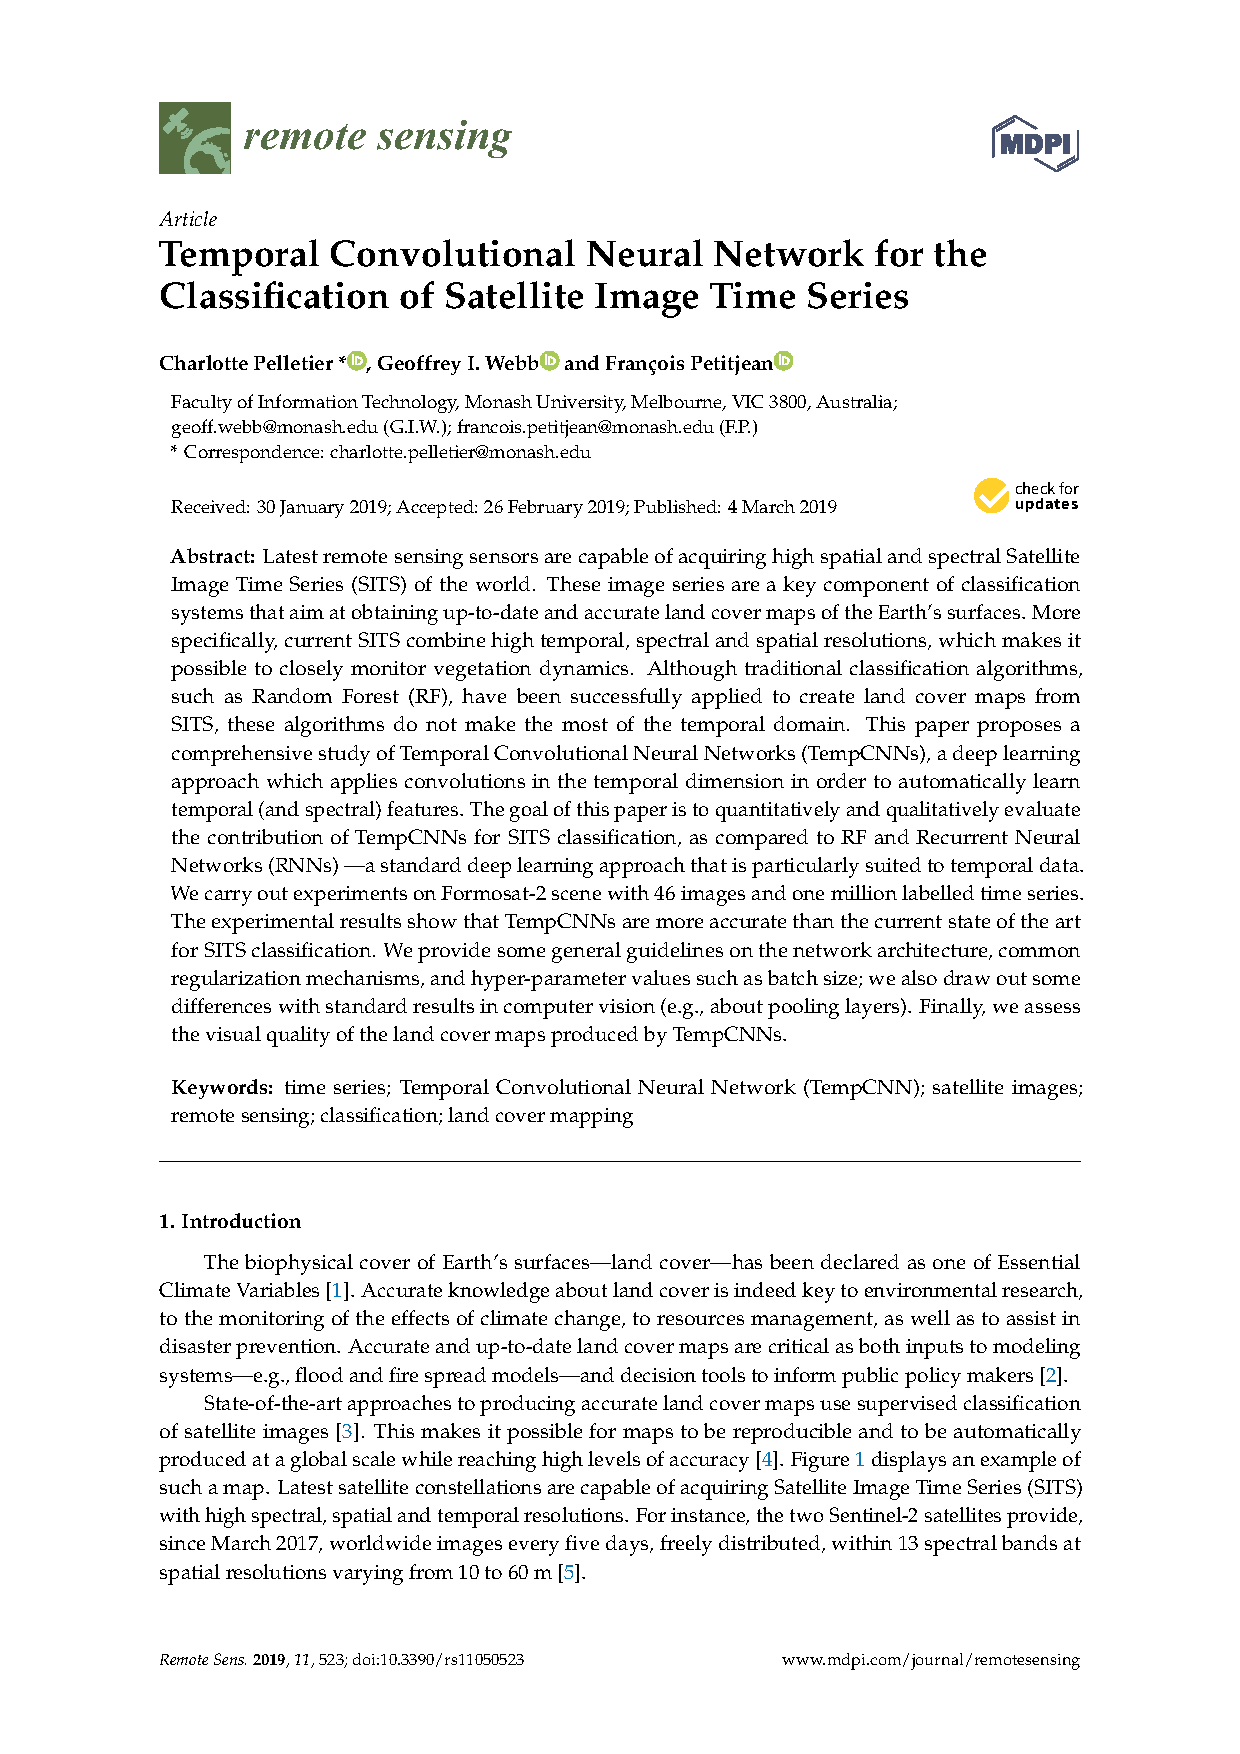
\includegraphics[width=1\textwidth]{tempCNN}
  \caption{Proposed temporal Convolutional Neural Network (TempCNN). The network input is a
  multi-variate time series. Three convolutional filters are consecutively applied, then one dense layer,
  and finally the Softmax layer, that provides the predicting class distribution.    \cite{tempCNN}}
  \label{tab:temCNNArchitecture}
\end{figure}


To prevent overfitting, we employed the same regularization mechanisms described in \cite{tempCNN}:

\begin{itemize}
  \item dropout rate of 0.5 \cite{JMLR:v15:srivastava14a}. 
  \item L2-regularization on the weights (also named weight-decay) applied for all the layers with a small rate of $10^{-6}$ 
  \item batch normalisation \cite{DBLP:journals/corr/IoffeS15}.
\end{itemize}

To train the network Adam optimization was used with the standard parameter values: $\beta_1 = 0.9$, $\beta_2 = 0.999$, and $e = 10^{-8}$) \cite{kingma2014adam} 
We used a batch size of 32, and a maximum number of epochs set to 20, with an early stopping mechanism with a patience of zero on the validation loss. 


\subsection{Experimental results}

In this section, we report the results of our experiments evaluating the performance of the TempCNN model on satellite image time series data.
We analyzed the effect of the depth of the network and the width of its convolutional layers on the classification accuracy.
Additionally, we investigated the effect of using different regularization techniques on the classification accuracy.
Finally, we investigated the effect of batch size on classification accuracy. 
By thoroughly investigating these factors, we gained insight into how to optimize the TempCNN model for this type of data.


\begin{paragraph}{Depth}
In a convolutional neural network (CNN), the depth refers to the number of layers in the network.
A deeper network can learn more complex features by using a hierarchy of layers, each building on the features learned by the previous layer.
However, increasing the depth can also lead to the vanishing gradient problem, where the gradients become too small to effectively update the weights during training.
Therefore, finding the optimal depth is a crucial consideration when designing a CNN.
\end{paragraph}

To investigate the impact of network depth on model performance while maintaining constant complexity, we vary the number of layers in the network while reducing the number of units in deeper layers.
We experiment with six architectures that consist of between one and six convolutional layers, each with a varying number of units ranging from 256 to 16.
Additionally, each architecture includes one dense layer with a number of units ranging from 64 to 2048. 
In each experiment, we train the model twice: first using the dataset with pre-imputed missing values, and then using a modified dataset where any missing values are replaced with zeros.
As shown in Table \ref{tab:temCNNdepth}, the highest accuracy is achieved with two or three convolutional layers.

\begin{table}[!htbp]
  \centering
   \begin{tabular}{rclrr}
   Model&&                  & No imputation         & Pre imputation             \\[0.2cm]
   \hline \\[-0.2cm]
   1CONV256 &+& 1FC64   	 & $91.39 \pm 0.74$ 	 & $91.12 \pm 0.57$\\
   2CONV128 &+& 1FC128  	 & $91.32 \pm 1.11$ 	 & $91.32 \pm 1.28$\\
   3CONV64 &+& 1FC256   	 & $\mathbf{92.57 \pm 0.84}$ 	 & $\mathbf{92.93 \pm 1.50}$\\
   4CONV32 &+& 1FC512   	 & $92.33 \pm 1.32$ 	 & $90.45 \pm 1.98$\\
   5CONV16 &+& 1FC1024  	 & $91.20 \pm 0.94$ 	 & $88.20 \pm 2.95$\\
   6CONV8 &+& 1FC2048   	 & $87.83 \pm 2.89$ 	 & $88.58 \pm 2.90$\\
   \end{tabular}
   \caption{Influence of depth on classification accuracy.}
   \label{tab:temCNNdepth}
 \end{table}

\begin{paragraph}{Width}
The width of a convolutional neural network (CNN) refers to the number of neurons in each layer.
Increasing the width can enhance the network's ability to learn complex features because more neurons are available for training.
However, a network that is too wide may be prone to overfitting, where it memorizes the training data rather than generalizing to new data.
Therefore, finding the optimal width is critical for achieving the best performance on the test data.
\end{paragraph}

To evaluate the impact of width on model performance, we experimented with seven CNN architectures.
Each architecture includes three convolutional layers, one dense layer with 256 neurons, and a Softmax layer, as illustrated in Figure \ref{tab:temCNNwidth}.
The architectures differ in the number of parameters, and we vary the width of the convolutional layers from 16 to 1024 neurons.

 \begin{table}[!htbp]
  \centering
   \begin{tabular}{rclrr}
   Model&&                  & No imputation         & Pre imputation             \\[0.2cm]
   \hline \\[-0.2cm]
   3CONV16 &+& 1FC256    	 & $92.44 \pm 0.83$ 	 & $91.62 \pm 0.41$\\
   3CONV32 &+& 1FC256    	 & $92.52 \pm 0.68$ 	 & $92.16 \pm 0.68$\\
   3CONV64 &+& 1FC256    	 & $92.45 \pm 0.89$ 	 & $\mathbf{93.47 \pm 0.63}$\\
   3CONV128 &+& 1FC256   	 & $92.26 \pm 1.84$ 	 & $92.13 \pm 1.35$\\
   3CONV256 &+& 1FC256   	 & $91.66 \pm 1.96$ 	 & $92.04 \pm 1.67$\\
   3CONV512 &+& 1FC256   	 & $91.97 \pm 1.23$ 	 & $92.75 \pm 1.73$\\
   3CONV1024 &+& 1FC256  	 & $\mathbf{92.76 \pm 1.46}$ 	 & $93.39 \pm 1.54$\\
   \end{tabular}
   \caption{Influence of width on classification accuracy.}
   \label{tab:temCNNwidth}
 \end{table}

The results reported in Table \ref{tab:temCNNwidth} show that the architecture is remarkably robust, even when there is considerable variation in the number of neurons. This is illustrated by the fact that the overall accuracy shows a difference of only 1.7\% between the model with lower parameters and the one with higher parameters when using pre-imputed data, while the difference is only 0.32\% when there is no imputation for missing values.
Although the standard deviation increases with the number of parameters, the architecture consistently achieves high accuracy rates, indicating that it is capable of maintaining good performance even with a larger number of neurons.

We opted to utilize the model with three convolutional layers, each with 64 neurons, and one dense layer comprising 256 neurons for the upcoming experiments because it offers a favorable balance between bias and variance. This choice was made with consideration to the size of our training dataset, which comprises 80,000 samples.

\begin{paragraph}{Batch size}
In machine learning, batch size refers to the number of training examples used in an iteration of gradient descent.
The batch size plays a crucial role in determining the efficiency and accuracy of the training process.
A larger batch size can result in faster training because the algorithm can process more examples in each iteration.
However, using a larger batch size can also lead to a less accurate model because it can cause the optimization algorithm to converge to a suboptimal solution.
On the other hand, using a smaller batch size may result in slower training, but may help the algorithm converge to a better solution. 
Thus, choosing an appropriate batch size is an important consideration in machine learning.
\end{paragraph}

We conducted experiments to determine the optimal batch size for training the TempCNN model.
Specifically, we tested four different batch sizes: 16, 32, 64, and 128.
Our analysis, as presented in Table \ref{tab:temCNNbatchsize}, shows that batch size has a noticeable impact on training time; larger batch sizes result in faster training times.
However, we observed that the batch size does not have a significant effect on the overall accuracy of the TempCNN model.
In fact, we found that the accuracy values for all four batch sizes are comparable, indicating that selecting an appropriate batch size is not a critical factor in achieving high accuracy for this model.

\begin{table}[!htbp]
  \centering
   \begin{tabular}{rlll}
   Batch size                 & Train time  & No imputation         & Pre imputation             \\[0.2cm]
   \hline \\[-0.2cm]
    16        & 52min  	 & $91.92 \pm 1.50$ 	 & $92.16 \pm 1.75$\\
    32        & 42min  	 & $\mathbf{91.61 \pm 1.19}$ 	 & $\mathbf{93.74 \pm 0.03}$\\
    64        & 26min  	 & $90.88 \pm 1.63$ 	 & $92.30 \pm 0.89$\\
    128       & 20min  	 & $91.54 \pm 1.69$ 	 & $91.52 \pm 1.67$\\
   \end{tabular}
   \caption{Influence of batch size on training time and classification accuracy.}
   \label{tab:temCNNbatchsize}
 \end{table}
 
\begin{paragraph}{Pooling layers}
Pooling is a common technique used in deep learning for dimensionality reduction and feature extraction.
In the context of computer vision, the two most popular types of pooling are local max-pooling \cite{Ren2015Faster} and global average pooling \cite{He2016Deep}.
Local max-pooling takes the maximum value of a small subregion of a feature map, while global average pooling takes the average of all feature map values.
However, for time series data, global average pooling has been shown to be more effective in previous studies \cite{rs10020236,fawaz2018deep}.
In this work, we investigate whether these findings can be generalized to time series classification tasks. 
Specifically, we will compare the performance of the TempCNN model using both local max-pooling and global average pooling to determine which pooling method is most effective for our specific application.
\end{paragraph}

\begin{paragraph}{Filter size}
Filter Size is an important Hyperparameter in Convolutional Neural Networks (CNNs)
The filter size, also known as the kernel size, determines the receptive field of the convolutional layer and influences the network's ability to capture spatial features in the input.
A larger filter size allows the network to capture more complex patterns and details, but at the cost of increased computation and potential overfitting.
Conversely, a smaller filter size reduces computation and may improve the network's ability to generalize to new data, but at the risk of losing important features.
Therefore, the filter size should be chosen based on the complexity of the task and the size of the input data.
\end{paragraph}


% TODO review
Figure \ref{tab:tempCNNPooling} displays the OA values as a function of filter size. 
Each bar represents a different configuration: local max-pooling (MP), local max-pooling and global average pooling (MP + GAP), local average pooling (AP), local and global average pooling (AP + GAP), and global average pooling (GAP). 
The horizontal magenta dashedline corresponds to the OA values obtained without pooling layers in the previous experiment.


\begin{figure}[!htbp]
  \centering
  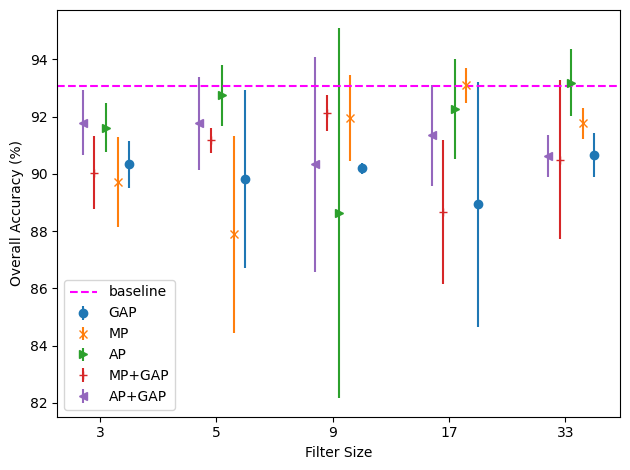
\includegraphics[width=0.7\textwidth]{tempCNNPooling.png}
  \caption{Overall Accuracy as a Function of Filter Size for Different Pooling Methods: Local max-pooling (MP) in orange, local max-pooling and global average pooling (MP + GAP) in red, local average pooling (AP) in green, local and global average pooling (AP + GAP) in purple, and global average pooling (GAP) in blue.}
  \label{tab:tempCNNPooling}
\end{figure}

Figure \ref{tab:tempCNNPooling} shows that the use of pooling layers performs poorly: the OA results are almost always
below the one obtained without pooling layers (magenta dashed line). 

% TODO ? Let us describe in more details thedifferent findings for both global and local pooling layers.



% TODO review architecture 
\pagebreak
\section{AJ-RNN}
``Adversarial Joint-Learning Recurrent Neural Network for Incomplete Time Series Classification" \cite{ajrnn} is a research paper that proposes a novel approach for classification of incomplete time series data.
The authors begin by highlighting the challenges of working with incomplete time series data, particularly the difficulty of extracting features and the need to deal with missing values.

To address these challenges, the authors propose an adversarial joint-learning recurrent neural network (AJ-RNN) that uses a recurrent neural network (RNN) to capture the temporal dependencies in the time series data, and an adversarial learning approach to impute the missing values.

The AJ-RNN is trained using a joint optimization framework that alternates between training the RNN for classification and the imputation network to fill in the missing values.
The adversarial component of the imputation network is used to ensure that the imputed values are as close as possible to the true values.

The authors evaluate the performance of the AJ-RNN on several real-world datasets and demonstrate that it outperforms several existing state-of-the-art approaches for time series classification.

\subsection{Adversarial learning}

% TODO review
Previous studies have shown that adversarial approaches outperform traditional methods in generating data that conforms to the distribution of a given dataset \cite{goodfellow2014generative, ledig2017photo}.

Furthermore, GANs have shown promising results in filling in missing data in time series prediction \cite{yoon2018gain, li2018learning, luo2018multivariate}. Similarly, adversarial techniques have also been applied to tasks such as video captioning \cite{yang2018video} and domain adaptation \cite{ganin2017domain}.
However, prior to this paper, the question of how to apply adversarial learning in the domain of incomplete time series classification (ITSC) has not been explored.

The integration of adversarial training and joint learning in recurrent neural networks (RNNs) is explored in this paper, resulting in the development of a system called Adversarial Joint learning RNN (AJ-RNN).

The study's results show that employing AJ-RNN, an end-to-end framework integrating adversarial training and joint learning in recurrent neural networks, is an effective solution to tackle the issue of incomplete time series classification.
J-RNN is trained to predict the value of the next input variable when it is revealed, and to fill in the missing value with its prediction.
At the same time, AJ-RNN also learns to classify.
Hence AJ-RNN can directly perform classification with missing values.

\subsection{Model}

% TODO rephrase

The following section presents the Adversarial Joint learning Recurrent Neural Network (AJ-RNN) as a solution for time series classification with missing values. 
The architecture of the model is illustrated in Figure \ref{fig:AJRNNrchitecture}. 

Here we describe how adversarial and joint learning strategies are integrated into an RNN.


The time series $X$ is represented as a sequence vector of $T$ observations, denoted by $X = \{x_1, x_2, ..., x_T \}$. Each observation $x_t \in R^d$ is a $d$-dimensional vector.

Assume that a time series $X$ has missing values which are represented by a $T$-dimensional mask vector $M = \{m_1, m_2, ..., m_T\}$.
The elements $m_t$ of the mask vector are binary values indicating the presence or absence of the corresponding element $x_t$ in the time series, where $m_t$ takes the value of $1$ if $x_t$ is revealed and $0$ if $x_t$ is missing.

Each time series $X^i$ in the dataset $D$ is associated with a target label $y^{(i)}$, and a mask vector $M^i$, where $D = {(X^i,M^i, y^i)}^N_{i=1}$.

To avoid the traditional two-step approach, imputation and classification are regarded as two tasks in multitask learning.

The AJ-RNN is trained to approximate the value of the next input variable and use it as a target when it is revealed.
If the next value is missing, it is filled in with the current prediction.
At the same time, the AJ-RNN is trained to perform the classification task.

The missing value problem is addressed through two processes, namely approximation and imputation.
As shown in Figure \ref{fig:AJRNNrchitecture}, two kinds of links enable AJ-RNN to directly model time series in the presence of missing values: dashed blue links (for approximation) and solid blue links (for imputation). 
The system is trained to approximate the next value $x_t$ using the last hidden state $h_{t-1}$ as follows:

\begin{equation}
  \hat{x_t} = W_{imp} h_{t-1} + b_z
\end{equation}

where $W_{imp} \in R^{n \times  m}$ is a learned regression matrix and $b_z$ is a bias term. 
As $\hat{x_t}$ is trained to approximate the next value $x_t$, it can be employed for imputing it when it is missing.
The input value $u_t$ is computed as:

\begin{equation}
  u_t = m_t \odot x_t + (1 - m_t) \odot \hat{x_t}
  \label{eq:AJRNNinput}
\end{equation}

where $m_t$ is the mask as defined above and $\odot$ is the element-wise product.

The completed input value $u_t$ is used to train the RNN.
The update equation of the RNN is:

\begin{equation}
  h_t = F_{RNN} (h_{t-1}, u_t; W)
\end{equation}

Where $h_t$ represents the hidden unit vector at time $t$, $W$ encapsulates the input-to-hidden and hidden-to-hidden parameters, and $F_{RNN}$ represents the update function of the particular RNN variant.

To obtain the probability distribution over each category label, a softmax is applied to the output of the classifier, which takes the last hidden state of the RNN, $h_T$, as input.

\begin{equation}
  P(\hat{y_j}|h_T ) = \frac{exp(W^T_j  h_T )}{\sum_{l=1}^K exp(W^T_l  h_T )}
  \label{eq:AJRNNsoftmax}
\end{equation}

where $K$ is the number of class labels and $\{W_l\}^K_{l=1}$ are the class-specific weights of the softmax layer.
More complex networks can be used for the classifier based on the specific task at hand. However, in this study, a simple classifier is used.
% TODO include ?
%to mainly demonstrate the mitigation of the exploding bias problem and to report the achieved results.
% For fairness, we use this approach for all methods, ours and the methods we implemented for comparison.

% TODO review


During joint learning, imputation and classification tasks are performed. 
Let $D$ be the time series dataset and let the superscript $i$ denote the $i$-th sample in the dataset.
The imputation task produces an imputation sequence vector $\hat{X^i} = { \hat{x}^i_2, ..., \hat{x}^i_T }$ for the $i$-th time series sample.
This vector is composed of two parts: approximation values (represented by orange units in Fig. \ref{fig:AJRNNrchitecture}) and imputation values (represented by purple units in Fig. \ref{fig:AJRNNrchitecture}).  
The imputation loss of all time series samples is calculated on the approximation values as follows:

\begin{equation}
  \mathcal{L}_{imp}(X, \hat{X}, M) = \frac{1}{N} \sum_{i=1}^N \lVert (X^i_{2:T} - \hat{X}^i) \odot M^i_{2:T} \rVert_2^2
  \label{eq:AJRNNimploss}
\end{equation}

where $N$ represents the number of samples in the dataset.
Equation (\ref{eq:AJRNNimploss}) measures the mean squared error loss between the approximation and the revealed values.
The mask $M^i_{2:T}$ is used to ignore the imputation values in the loss calculation, as there is no ground truth available for these missing values.


The loss for the classification task can be calculated as follows. 
Let $y^i$ be the true label of the $i$-th time series sample and $\hat{y}^i$ be the predicted probability distribution given by Equation (\ref{eq:AJRNNsoftmax}).

\begin{equation}
  \mathcal{L}_{cls}(y, \hat{y}) = - \frac{1}{N} \sum_{i=1}^N \sum_{j=1}^K 1\{ y^i = j\} \log\hat{y}^i 
  \label{eq:AJRNNclsloss}
\end{equation}

where $K$ represents the number of class labels. 
Equation (\ref{eq:AJRNNclsloss}) is the softmax cross entropy loss of the predicted label and the true label.

The end-to-end framework is susceptible to the negative impact of missing values, which can propagate errors from the imputation task to the classification task.
The imputed values are predictions and are prone to errors, which can quickly amplify as they are fed into the RNN, leading to the problem of exploding bias.

Here, a discriminator $D$ is introduced to alleviate the negative impact of missing values.  
Unlike the traditional approach that identifies the entire completed vector, the discriminator $D$ distinguishes whether each value in the completed vector is real or imputed.
This direct supervision of the imputed values by the discriminator $D$ can help reduce the error propagation from imputation to classification.

Specifically, for each training sample $i$ in the time series dataset, there exists a completed sequence vector $U^i = {u^i_2 , ..., u^i_T}$ obtained through Equation (\ref{eq:AJRNNinput}), along with its corresponding mask vector $M^i_{2:T} = {m^i_2, ..., m^i_T }$.

In $U^i$, some are real values, while the rest are imputed.
We know which are which by the mask vector $M^i$.
We can take advantage of this knowledge to provide a supervision signal for the imputation network.

The adversarial learning strategy involves two players in a minimax game: the discriminator $D$ and the AJ-RNN \footnote{RNN and Classifier}.
The parameters of both models are updated alternately.
Initially, the discriminator $D$ takes the completed sequence vector as input and is trained to distinguish between the revealed and imputed values in the vector.
The discriminator loss can be defined as follows:

\begin{align}
  \mathcal{L}_{D}(U, M) & = - [E \log(D(X_{real})) + E \log(1 - D(\hat{X}_{imp}))] \label{eq:AJRNNdloss} \\ 
                        & = - \frac{1}{N} \sum_{i=1}^N \left[ M^i_{2:T} \odot \log(D(U^i)) + (1 - M^i_{2:T}) \odot \log(1-D(U^i)) \right]
\end{align}

Here, the function $D(\cdot)$ takes in the completed sequence vector as input and outputs the estimated mask probability $\hat{P}$ of the discriminator.
 
In Equation (\ref{eq:AJRNNdloss}), the first term is the log output of the discriminator on real values, and the discriminator tries to maximize this to 1.
The second term is the loss for imputed values.
Hence the discriminator tries to minimize its output for imputed values.

The discriminator is designed as a neural network composed of three fully connected layers to leverage global contextual information from the input sequence.
The first hidden layer has $T$ units, which is equal to the length of the input sequence, the second hidden layer has $T/2$ units, and the third hidden layer has $T$ units. 
The activation function used in each layer is the hyperbolic tangent (tanh) except for the output layer, where the sigmoid activation function is used to obtain the estimated probability of each value being real or fake.

The goal of the RNN is to minimize the difference between the distribution of predicted values and the distribution of revealed ones by deceiving the discriminator $D$. 
This provides a supervisory signal to the imputation network to produce better imputed values. 

The adversarial loss of the RNN can be defined as follows:

\begin{equation}
  \mathcal{L}_{adv}(U, M) = \frac{1}{N} \sum_{i=1}^N  (1 - M^i_{2:T}) \odot \log(1 - D(U^i))
  \label{eq:AJRNNadvloss}
\end{equation}

Hence the AJ-RNN tries to maximize the discriminator output for imputed values.
This provides a supervisory signal for each imputed value in the completed sequence vector, which can reduce the bias introduced by the imputation operation and thus alleviate the exploding bias problem.
Note that we can also feed the whole imputation vector $\hat{X}^i$ into the discriminator, providing supervision for both the approximated and imputed values. 
However, in practice, using only the imputed values is more computationally efficient and yields similar results as using both approximated and imputed values. 
Hence, considering computational efficiency, Equation (\ref{eq:AJRNNadvloss}) was we adopted as the adversarial loss.

Finally, the overall training loss of AJ-RNN is defined as follows:

\begin{equation}
  \mathcal{L}_{AJ-RNN} = \mathcal{L}_{cls} + \mathcal{L}_{imp} + \lambda_d \mathcal{L}_{adv}
  \label{eq:AJRNNloss}
\end{equation}

where $\lambda_d$ is hyper-parameter. 
This forms an end-to-end training framework for incomplete time series classification.

AJ-RNN combines the merits of joint learning and adversarial learning.
The discriminator $D$ is trained with the revealed values and the mask vector effectively provides supervision on each imputed value. 
Therefore, the negative impact of missing values on AJ-RNN is reduced.

\begin{figure}[H]
  \centering
  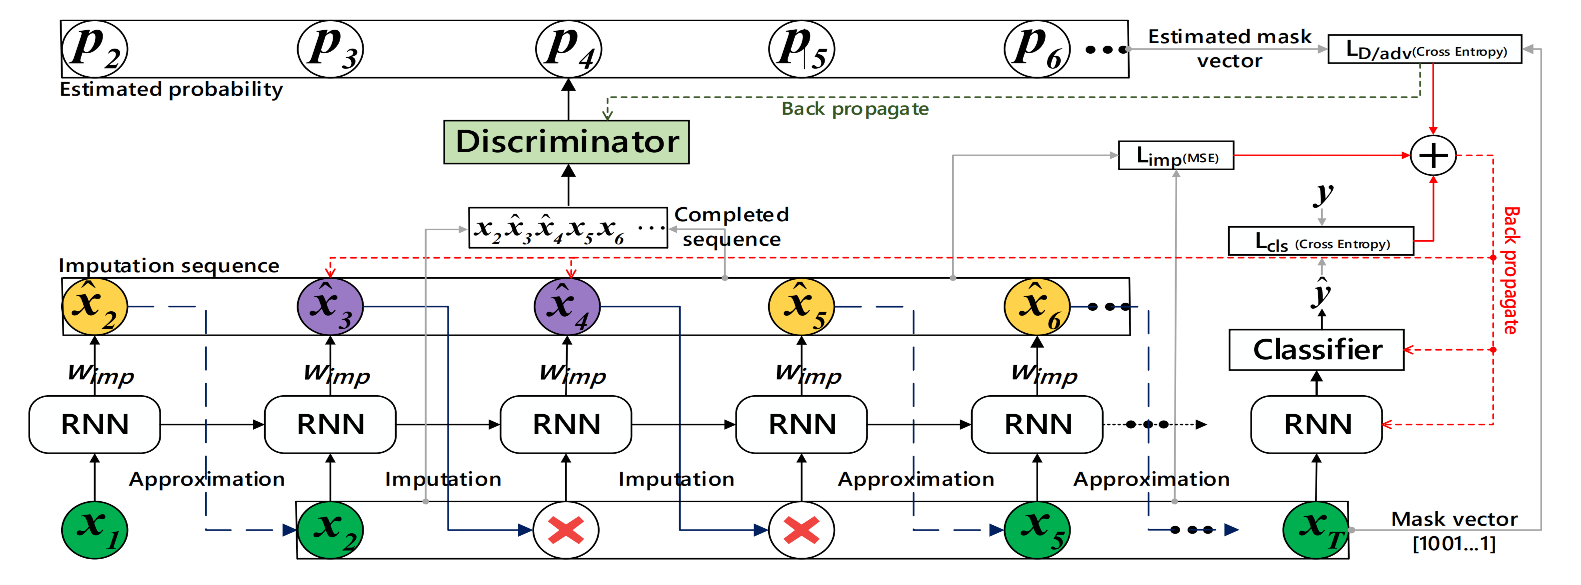
\includegraphics[width=1\textwidth]{ajrnn}
  \caption{The figure shows the proposed AJ-RNN framework. The green units represent revealed inputs, yellow for the output of approximated values, purple for the imputed values, and a red "X" for missing inputs. The dashed links represent the approximation training, while the solid links represent imputation. The discriminator receives a completed vector composed of revealed and imputed values as input, which provides a one-to-one supervisory signal for imputed values $\hat{x_3}$ and $\hat{x_4}$.}
  \label{fig:AJRNNrchitecture}
\end{figure}

\subsection{Data preparation}
As described in Section \ref{sec:tempCNNDataPreparation}, we divided our dataset into three separate subsets, namely training, validation, and test, in a 60:20:20 ratio, respectively. 
Our goal was to ensure that each subset had a similar class distribution and that there was no spatial autocorrelation between them.

We understood the significance of the mask vector in the AJ-RNN model, which is used to differentiate between revealed and imputed values.
Therefore, we generated a mask vector for each sample to feed into the model.

\subsection{Experimental results}

The AJ-RNN model proposed in the paper was implemented in Python 2.7 and Tensorflow 1.0.
However, given the changes in technology and advances in the field since the publication of the paper, we found it necessary to re-implement the model in a more recent version of TensorFlow.
As such, we spent a considerable amount of time and effort to re-implement the model in Tensorflow 2.0 in a modularized fashion, with the aim of enhancing code readability and facilitating experimentation with different configurations.

In addition to the re-implementation of the model, we also performed a careful validation process to ensure that the accuracy achieved by our model was consistent with the results reported in the original paper, using the same datasets. 
This involved testing the model on a range of datasets and comparing the results with the original paper. 
By doing so, we were able to ensure that our implementation was both accurate and reliable.

Furthermore, we extended the implementation of the model to support multivariate time series data. 
This undertaking was quite significant as it required extensive additional coding and validation efforts. 
However, it was essential to ensure that the AJ-RNN model could be effectively utilized in various applications, including our own.


We tried different combinations of hyper-parameters to find the best configuration for our dataset.
The hyper-parameters we tuned are the RNN cell type, the units of the cell, the learning rate, the batch size, and the number of epochs for the generator and discriminator.

In our experiments, we investigated the performance of the AJ-RNN model with both LSTM and GRU cells. 
We tested different numbers of units (64, 128) and dropout rates (0.2, 0.4, 0.6, 0.8) for each cell type. 
The experimental results are summarized in Table \ref{tab:AJRNNcelltype}. 
A learning rate of 0.001 and a batch size of 256 were used in all experiments, and the generator and discriminator were trained for the same number of epochs. 
Our findings show that the GRU cell outperforms the LSTM cell in all cases.

\begin{table}[H]
  \centering
  \begin{tabular}{cccr} 
      Cell type & Units & Dropout & Overall Accuracy\\[0.2cm] 
      \hline \\[-0.2cm] 
      GRU   &   64  & 0.2 &  $82.10 \pm 1.72$\\
      GRU   &   64  & 0.4 &  $81.75 \pm 1.18$\\
      GRU   &   64  & 0.6 &  $77.70 \pm 2.92$\\
      GRU   &   64  & 0.8 &  $78.78 \pm 2.26$\\[0.05cm] \hline \\[-0.25cm]

      GRU   &   128 & 0.2 &  $80.58 \pm 1.17$\\
      GRU   &   128 & 0.4 &  $85.84 \pm 1.68$\\
      GRU   &   128 & 0.6 &  $\mathbf{86.07 \pm 1.58}$\\
      GRU   &   128 & 0.8 &  $85.03 \pm 2.66$\\[0.05cm] \hline \\[-0.25cm]

      GRU   &   256 & 0.2 &  $80.49 \pm 1.47$\\
      GRU   &   256 & 0.4 &  $75.25 \pm 1.08$\\
      GRU   &   256 & 0.6 &  $75.97 \pm 1.23$\\
      GRU   &   256 & 0.8 &  $77.34 \pm 1.74$\\[0.05cm] \hline \\[-0.25cm]

      LSTM  &   64  & 0.2 &  $79.41 \pm 1.76$\\
      LSTM  &   64  & 0.4 &  $84.92 \pm 3.69$\\
      LSTM  &   64  & 0.6 &  $81.16 \pm 2.99$\\
      LSTM  &   64  & 0.8 &  $79.56 \pm 2.33$\\[0.05cm] \hline \\[-0.25cm]

      LSTM  &   128 & 0.2 &  $84.89 \pm 1.56$\\
      LSTM  &   128 & 0.4 &  $85.08 \pm 0.35$\\
      LSTM  &   128 & 0.6 &  $83.24 \pm 1.29$\\
      LSTM  &   128 & 0.8 &  $82.39 \pm 1.99$\\[0.05cm] \hline \\[-0.25cm]

      LSTM  &   256 & 0.2 &  $74.18 \pm 1.44$\\
      LSTM  &   256 & 0.4 &  $67.15 \pm 1.32$\\
      LSTM  &   256 & 0.6 &  $71.36 \pm 1.56$\\
      LSTM  &   256 & 0.8 &  $\mathbf{85.37 \pm 2.37}$\\ 
      
  \end{tabular}
  \caption{Overall Accuracy for GRU and LSTM.}
  \label{tab:AJRNNcelltype}
\end{table}

After conducting experiments with both LSTM and GRU cells with varying numbers of units and dropout rates, we determined that the GRU cell outperformed the LSTM cell.
As a result, we chose to further experiment with the GRU cell. 
We found that using a GRU cell with 128 units was a good compromise between model complexity and accuracy. 
This decision was made after careful consideration of the trade-off between the number of parameters in the model and its ability to accurately classify incomplete time series data.

We also investigated the effect of batch size on the overall accuracy of the model.
We tried different batch sizes and found that the batch size of 256 yielded the best results.
The results are summarized in Table \ref{tab:AJRNNbatchsize}.

\begin{table}[H]
  \centering
  \begin{tabular}{cccr} 
      Batch size & Learning rate & Dropout & Overall Accuracy\\[0.2cm] 
      \hline \\[-0.2cm]
      256 &   1e-03 &   0.0 & $80.13 \pm 2.20$\\
      256 &   1e-03 &   0.2 & $81.58 \pm 1.17$\\
      256 &   1e-03 &   0.4 & $85.85 \pm 1.39$\\
      256 &   1e-03 &   0.6 & $\mathbf{86.03 \pm 1.51}$\\
      256 &   1e-03 &   0.8 & $84.03 \pm 2.66$\\[0.05cm] \hline \\[-0.25cm]

      256 &   1e-04 &   0.4 & $80.00 \pm 1.91$\\
      256 &   1e-04 &   0.6 & $85.46 \pm 1.01$\\
      256 &   1e-04 &   0.8 & $83.88 \pm 1.33$\\[0.05cm] \hline \\[-0.25cm]

      32  &   1e-03 & 0.0 & $35.57 \pm 0.00$\\
      32  &   1e-03 & 0.5 & $29.32 \pm 0.00$\\[0.05cm] \hline \\[-0.25cm]

      32  &   1e-04 & 0.0 & $35.58 \pm 4.65$\\
      32  &   1e-04 & 0.5 & $36.27 \pm 8.39$\\
      32  &   1e-04 & 0.8 & $35.58 \pm 2.33$\\[0.05cm] \hline \\[-0.25cm]

      32  &   1e-05 & 0.0 & $56.12 \pm 0.88$\\
      32  &   1e-05 & 0.5 & $69.33 \pm 0.34$\\
      32  &   1e-05 & 0.8 & $67.12 \pm 1.23$\\[0.05cm] \hline \\[-0.25cm]

      32  &   1e-06 & 0.0 & $64.06 \pm 2.74$\\
      32  &   1e-06 & 0.5 & $66.58 \pm 3.78$\\[0.05cm] \hline \\[-0.25cm]

      32  &   1e-07 & 0.0 & $72.97 \pm 1.56$\\
      32  &   1e-07 & 0.5 & $71.70 \pm 1.45$\\[0.05cm] \hline \\[-0.25cm]

      32  &   1e-08 & 0.0 & $73.85 \pm 1.31$\\
      32  &   1e-08 & 0.5 & $72.92 \pm 1.40$\\[0.05cm] \hline \\[-0.25cm]

      32  &   1e-09 & 0.0 & $\mathbf{77.24 \pm 1.12}$\\
      32  &   1e-09 & 0.5 & $76.37 \pm 1.36$\\
  \end{tabular}
  \caption{Influence of batch size, learning rate and dropout on Overall Accuracy for the GRU network}
  \label{tab:AJRNNbatchsize}
\end{table}

During our experiments, we observed that the choice of batch size has a significant impact on the accuracy of the model, when the learning rate is was constant.
Specifically, we found that using a smaller batch size can increase the likelihood of over fitting the training data, while using a larger batch size can lead to under fitting.

To improve the overall accuracy of the model with a lower batch size, we attempted to decrease the learning rate.
However, while we did observe some improvement, we were not able to achieve the same level of accuracy as when using a higher batch size.
These findings highlight the importance of carefully selecting hyperparameters, such as batch size and learning rate, to achieve optimal performance in machine learning models.

We also explored the impact of increasing the number of the generator $G$ epochs for each training step.

\begin{table}[H]
  \centering
  \begin{tabular}{cccr} 
      Batch size & G epochs & Overall Accuracy\\[0.2cm] 
      \hline \\[-0.2cm]
      256 &   1 &  $\mathbf{86.03 \pm 1.51}$\\
      256 &   2 &  $72.58 \pm 1.17$\\
      256 &   5 &  $68.05 \pm 1.39$\\[0.05cm] \hline \\[-0.25cm]
      32  &   1 &  $\mathbf{77.24 \pm 1.12}$\\
      32  &   2 &  $57.21 \pm 1.46$\\
      32  &   5 &  $27.07 \pm 1.05$\\
  \end{tabular}
  \caption{Influence of G epochs for the GRU network}
  \label{tab:AJRNNGepochs}
\end{table}

Our analysis revealed that augmenting the number of $G$ epochs can result in overfitting the training data, as presented in Table \ref{tab:AJRNNGepochs}.


\pagebreak
\subsection{Light AJ-RNN}

Due to the computational expense of the AJ-RNN model, we decided to conduct experiments with a lighter version of the model, referred to as the Light AJ-RNN.
The goal of this approach was to create a baseline model that could be used as a reference point for comparison with the more complex and computationally demanding AJ-RNN model. 

In order to achieve this, we used the Keras library to implement the Light AJ-RNN model.
Our approach involved removing the imputation of missing values from the original AJ-RNN model and utilizing the pre-imputed data as input to the model.
We removed the Discriminator and thus eliminated adversarial joint training.
The Light AJ-RNN model only retained the GRU network and the Classifier from the original AJ-RNN model.
This approach was aimed at achieving a reduction in computational costs while still maintaining a level of performance comparable to the original AJ-RNN model.

We conducted experiments with the Light AJ-RNN model using the same hyperparameters as the original AJ-RNN model.


\begin{table}[H]
  \centering
  \begin{tabular}{cccr} 
      Batch size & Learning rate & Dropout & Overall Accuracy\\[0.2cm] 
      \hline \\[-0.2cm]
      256 & 0.0 & 1e-03 & $75.14 \pm 1.85$\\
      256 & 0.5 & 1e-03 & $78.48 \pm 1.33$\\[0.05cm] \hline \\[-0.25cm]

      256 & 0.0 & 1e-04 & $87.25 \pm 1.20$\\
      256 & 0.5 & 1e-04 & $82.60 \pm 2.17$\\
      256 & 0.8 & 1e-04 & $\mathbf{87.29 \pm 1.08}$\\[0.05cm] \hline \\[-0.25cm]

      256 & 0.0 & 1e-05 & $83.29 \pm 2.85$\\
      256 & 0.0 & 1e-06 & $85.59 \pm 1.30$\\[0.05cm] \hline \\[-0.25cm]

      256 & 0.0 & 1e-07 & $81.72 \pm 1.32$\\
      256 & 0.5 & 1e-07 & $81.76 \pm 2.21$\\[0.05cm] \hline \\[-0.25cm]

      32  & 0.5 & 1e-03 & $30.85 \pm 1.35$\\[0.05cm] \hline \\[-0.25cm]

      32  & 0.0 & 1e-04 & $33.55 \pm 1.42$\\
      32  & 0.5 & 1e-04 & $32.33 \pm 1.33$\\[0.05cm] \hline \\[-0.25cm]

      32  & 0.0 & 1e-05 & $44.23 \pm 2.02$\\[0.05cm] \hline \\[-0.25cm]
      32  & 0.0 & 1e-06 & $54.32 \pm 3.73$\\[0.05cm] \hline \\[-0.25cm]
      32  & 0.0 & 1e-07 & $52.98 \pm 2.22$\\[0.05cm] \hline \\[-0.25cm]
      32  & 0.0 & 1e-08 & $\mathbf{55.80 \pm 1.27}$\\
      32  & 0.5 & 1e-08 & $52.32 \pm 1.36$\\
  \end{tabular}
  \caption{Overall accuracy of Light AJ-RNN model for different hyperparameters}
  \label{tab:LightAJRNNBatchSizeResults}
\end{table}

The results of the experiments are shown in Table \ref{tab:LightAJRNNBatchSizeResults}.

Despite our initial hopes that the Light AJ-RNN model would prove to be a viable alternative to the computationally expensive original AJ-RNN model, the results of our experiments showed that the overall accuracy of the Light AJ-RNN model was comparable to that of the original AJ-RNN model for most of the hyperparameter combinations tested.

Interestingly, despite using pre-imputed data as input to the model, we did not observe the expected improvement in overall accuracy that we had hoped for. 
While disappointing, this result was nonetheless informative and suggested that the original AJ-RNN model was indeed necessary for achieving the highest levels of accuracy in our application.

Therefore, we made the decision to halt further experimentation with the Light AJ-RNN model and instead focused our efforts on continuing to refine and improve the original AJ-RNN model. 


\subsection{Findings}

In the study conducted on the AJ-RNN model, a deep learning model for classifying time series while imputing missing data.
Our experiments aimed to explore the performance of the model and to find the best hyperparameters for our real-world dataset.

Overall, our findings were mixed. 
While the model showed promise on some of our experiments, we found that the overall accuracy on our real-world dataset was not as high as we expected.
It is worth noting that training RNNs is very computationally expensive, and we had to run many experiments to find the best hyperparameters.

We also found that the adversarial joint training is really sensitive to the hyperparameters.
We experimented with different learning rates, batch sizes, and dropout rates and found that these parameters can significantly impact the performance of the model.
Therefore, it is important to carefully tune these hyperparameters to achieve the best possible results.

In conclusion, we found that the AJ-RNN model can be an effective tool for imputing missing data. 
However, it is important to carefully consider the hyperparameters and to perform extensive experimentation to achieve the best possible results.

The model has been implemented in Python using the Keras library \cite{chollet2015keras} and the TensorFlow backend \cite{tensorflow2015-whitepaper}.
The source code for this model is accessible at \url{https://github.com/dnldsht/AJ-RNN}, which is a reimplemented and extended version of the initial AJ-RNN implementation \cite{ajrnn}.
\pagebreak
\section{L-TAE}
In order to embed the input images into the L-TAE model, we needed to replace the Pixel Set Encoder (PSE) used in the original model with an encoder that was more appropriate for our dataset.

This led to the adoption of the Dense Encoder (DE), which is a linear neural network that takes a 16-channel image as input and uses a hyperbolic tangent (tanh) activation function to generate a 64-dimensional vector.
Our goal in designing the DE was to ensure computational efficiency, allowing faster training and inference times, while maintaining strong performance on our dataset.

\subsection{Experimental results}

After adapting the L-TAE model to our dataset, we trained it by adjusting the hyperparameters to find the optimal configuration, guided by the results of their research.

\begin{table}[ht]
  \centering
  \begin{tabular}{l p{10cm}}   
     Param & Description \\[0.2cm] 
     \hline \\[-0.2cm]  
     E & size of the embeddings ($E$), if input vectors are of a different size, a linear layer is used to project them d\_model-dimensional space \\
     H & Number of attention heads  \\
     K & Dimension of the key and query vectors  \\
     MLP & Number of neurons in the layers of MLP \\
  \end{tabular}
  \caption{Hyper-parameters of L-TAE model}
  \label{tab:LTAEconfig}
\end{table}

In the following, we have described the findings of the authors on the impact of the different hyperparameters on the performance of the model.

\begin{paragraph} {Number of heads} 
It appears that the performance is only marginally impacted by the number of heads. 
Their hypothesis is that an increase in the number of heads ($H$) can be advantageous, but a reduction in group size ($E'$) can be detrimental.
\end{paragraph}

\begin{paragraph} {Dimension of keys}
The experiments indicate that smaller key dimensions, as opposed to the typical values used in NLP or for the TAE ($K = 32$), lead to better performance on the problem.
The L-TAE can achieve comparable performance to the TAE with only 2-dimensional keys.
\end{paragraph}

\begin{paragraph} {Dimension of Input}
The expected outcome of having larger input embeddings is an increase in performance, as it corresponds to a more comprehensive representation.
Nevertheless, on the dataset being considered, the benefits of increasing the number of parameters are diminishing.
\end{paragraph}

\begin{paragraph} {Query-as-Parameter}
To evaluate the impact of the design choices, a variation of the network is trained using the same master-query scheme as the TAE.
The larger linear layer that results increases the model's size to a total of 170k parameters.
The observation that the resulting mIoU is only 49.7 suggests that the query-as-parameter scheme is advantageous not only in terms of compactness but also for achieving better performance.
\end{paragraph}

Table \ref{tab:LTAEresults} shows the performance results of the L-TAE architecture with different configurations of the following hyperparameters: number of heads H, dimension of keys K, and number of channels E in the input sequence.
All results were obtained using a 5-fold cross-validation scheme.
The performance metrics were measured for two different scenarios: one where missing values were imputed and one where missing values were not imputed.

\begin{table}[H]
  \centering
  \begin{tabular}{cccclrr} 
     Params & E & H & K & MLP & No imputation & Pre imputation\\[0.2cm] 
     \hline \\[-0.2cm] 
     43k & 	128 & 	8 & 	8 & 	128 & 	$93.37 \pm 1.65$ & 	$93.08 \pm 1.16$\\ 
     68k & 	128 & 	16 & 	8 & 	128-128 & 	$93.43 \pm 1.37$ & 	$93.39 \pm 1.16$\\ 
     123k & 	256 & 	16 & 	8 & 	256-128 & 	$93.15 \pm 1.72$ & 	$93.44 \pm 1.22$\\ 
     299k & 	512 & 	32 & 	8 & 	512-128 & 	$\mathbf{93.65 \pm 1.30}$ & 	$93.40 \pm 1.16$\\ 
     749k & 	1024 & 	32 & 	8 & 	1024-256-128 & 	$92.91 \pm 1.90$ & 	$\mathbf{93.58 \pm 1.29}$\\ 
  \end{tabular}
  \caption{Results of the L-TAE model with different parameters}
  \label{tab:LTAEresults}
\end{table}

Overall, the results reported in Table \ref{tab:LTAEresults} demonstrate the effectiveness of the L-TAE architecture in accurately classifying the input data even with a lower number of parameters. 
The inclusion of missing data through imputation did not significantly impact the performance of the model, suggesting that the L-TAE architecture is robust to the presence of missing values.

The model has been implemented in Python using the PyTorch library \cite{NEURIPS2019_9015}.
The source code for this model is available at \url{https://github.com/dnldsht/lightweight-temporal-attention-pytorch}, which is a forked version of the orginal L-TAE implementation \cite{LTAE}.
\pagebreak

\section{Comparing results}

The performance of the different models on both the imputed and non-imputed datasets is compared in this section.

\begin{table}[H]
  \centering
    \begin{tabular}{lr}
    Model                       & Overall Accuracy             \\[0.2cm] 
    \hline \\[-0.2cm]
    RF            & $91.03 \pm 0.42$\\
    Light AJ-RNN  & $87.29 \pm 1.08$\\
    TempCNN       & $93.74 \pm 0.03$\\
    L-TAE         & $93.58 \pm 1.29$
    \end{tabular}
  \caption{Overall accuracy of the best models with pre imputed missing values}
  \label{tab:ALLresultsImputed} 
\end{table}

\begin{table}[H]
  \centering
    \begin{tabular}{lr}
    Model                       & Overall Accuracy             \\[0.2cm] 
    \hline \\[-0.2cm]
    RF      & $89.72 \pm 0.84$\\
    AJ-RNN  & $86.07 \pm 1.58$\\
    TempCNN & $92.57 \pm 0.84$\\
    L-TAE   & $93.65 \pm 1.30$
    \end{tabular}
  \caption{Overall accuracy of the best models without imputation of missing values} 
  \label{tab:ALLresultsNoImputed}
\end{table}

Overall, our experiments show that TempCNN and L-TAE outperformed the other models on both datasets.
Specifically, L-TAE achieved an accuracy of 93.58\% and 93.65\% on the imputed and non-imputed datasets, respectively, 
while TempCNN achieved an accuracy of 93.74\% and 92.57\%. RF and AJ-RNN both achieved lower accuracies. 
These results suggest that deep learning models such as TempCNN and L-TAE may be more suitable for modeling satellite image time series data.

\begin{figure}[H]
  \centering
  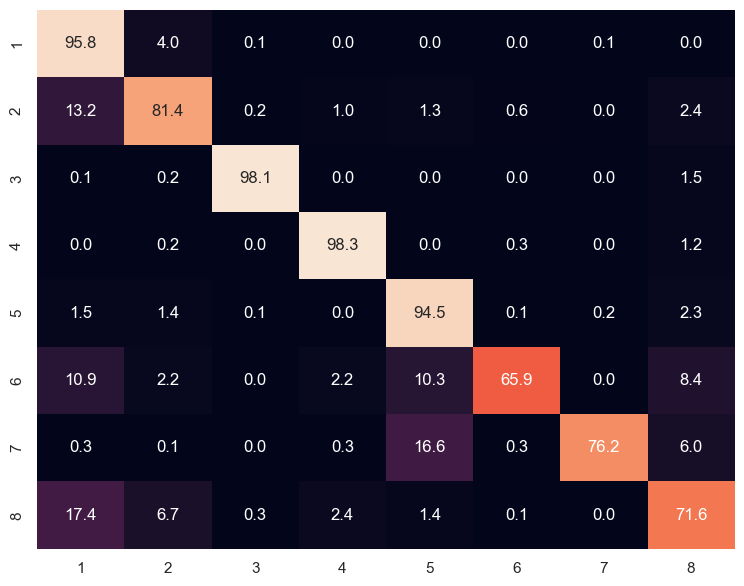
\includegraphics[height=5.14cm,width=0.47\textwidth]{cfTempCNN}
  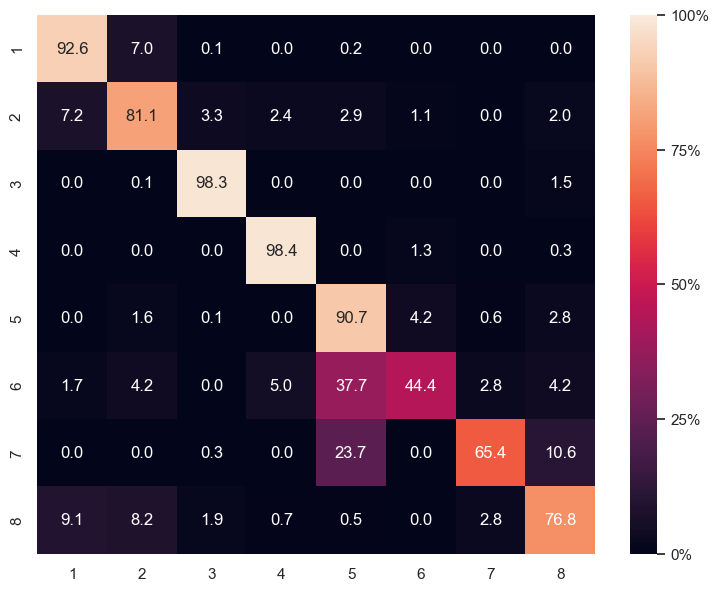
\includegraphics[width=0.52\textwidth]{cfLTAE}
  \caption{Confusion matrices for the TempCNN model (left) and L-TAE model (right) on the test dataset. The y-axis represents the true labels, and the x-axis represents the predicted labels.}
\end{figure}

Based on the confusion matrices, both TempCNN and L-TAE models seem to have difficulty distinguishing between the orchard and crop classes, as indicated by the high number of misclassifications between these two classes.
This could be due to the fact that these two classes may share similar temporal patterns in the time series data, making it more difficult for the models to distinguish between them. 
It may be worth exploring additional features or data sources to improve the performance of the models in distinguishing between these two classes.

\subsection{Imputation of missing values}

The inclusion of missing data is often a challenge in machine learning tasks, as missing values can have a significant impact on the performance of the model.
In the first scenario, we addressed this issue by imputing the missing values prior to training the models. 
This allowed us to utilize all available data in the training process, potentially leading to improved performance.

In the second scenario, we did not impute the missing values, which meant that the training process was performed using only the available non-missing data.
This scenario may be particularly useful in cases where imputation may introduce bias or distort the underlying patterns in the data.

Overall, the results reported in Tables \ref{tab:ALLresultsImputed} and \ref{tab:ALLresultsNoImputed} show that the inclusion of missing data through imputation did not significantly affect the performance of the models.